\cleardoublepage


\chapter{Inverse Kinematik}

In der direkte Kinematik wird aus den Gelenkzuständen Position und Rotation des Endeffektors bestimmt.
Der umgekehrte Vorgang, also das Berechnen der Gelenkpositionen bei gegebener Zieltransformation, wird als inverse Kinematik bezeichnet.
Dies ist erforderlich, um Aufgaben in der Umgebung des Roboters zu lösen und die angestrebten Zielpunkte zu erreichen.
Dabei muss beachtet werden, dass oft mehrere gleichwertige Lösungen für eine Zielstellung des Endeffektors vorliegen.
Allerdings kann die inverse Kinematik offener Ketten oft nicht einfach direkt mithilfe einer mathematischen Formel gelöst werden (siehe Abschnitt~\ref{sec:analytische-losung}).
Im Fall des UR5, ist dies allerdings in den meisten Fällen möglich.

Die Lösung des Problems kann geometrisch, analytisch oder numerisch gelöst werden.
Auf die ersten beiden Lösungsmöglichkeiten wird im Folgenden näher eingegangen.


\section{Analytische Lösung}\label{sec:analytische-losung}

Für eine direkte Lösung muss die Formel aus Gleichungen~\ref{eq:dh5} und~\ref{eq:subst2} herangezogen werden.
Nach Multiplikation der Transformationsmatrizen müsste die entstehende Gleichung~\ref{eq:inv-kin1} nach den Variablen $q_1$ bis $q_n$ aufgelöst werden.
Da aufgrund der rotatorischen Gelenke nichtlineare trigonometrische Funktionen verwendet werden, ist diese Funktion bei Industrierobotern meist nichtlinear und in vielen Fällen auch nicht lösbar.

\begin{equation}
    T_{0,n}(\overrightarrow{q}) = \prod_{i=1}^{n} T_{i-1,i}(q_i)     \label{eq:inv-kin1}
\end{equation}


\section{Geometrische Lösung}\label{sec:geometrische-losung}
Um die Berechnung zu vereinfachen, wird oftmals in den äußeren drei Gelenken eines Sechsarmroboters ein Handwurzelpunkt eingeführt, in dem sich die Achsgeraden dieser Gelenke schneiden.
Da die Drehung des sogenannten Handgelenks die Position des Handwurzelpunktes nicht verändert, kann so zuerst die Berechnung der Position des Handwurzelpunkts mithilfe der Zieltransformation und im Anschluss unabhängig die Berechnung der restlichen Gelenke stattfinden.
Dieser Trick ist allerdings im UR5 nicht verwendbar, da hier wohl aufgrund der größeren Zahl an Singularitäten dieser Technik (siehe Abschnitt~\ref{sec:singularitaten}) auf die Verwendung eines Handwurzelpunkts verzichtet wurde.

Dennoch kann durch eine Analyse der geometrischen Eigenschaften und der geringen Zahl der Singularitäten des UR5 eine Lösung von $\overrightarrow{q}$ bzw. $\overrightarrow{\theta}$ gefunden werden.
Die Strategie hierbei ist, beim ersten Gelenk zu beginnen und nach und nach die anderen Gelenke mit der Transformation $T_{0,6}$ des Endeffektors zu verknüpfen.
Bekannt sind zu Beginn der Rechnung nur die DH-Parameter $(\theta_i, a_i, d_i, \alpha_i)$ jedes Gelenks $i$ im Ausgangszustand, wobei $\theta_i$ als freie Variable jedes Gelenks betrachtet wird (Abschnitt~\ref{sec:ur5-in-dh}), sowie die Transformation des Endeffektors $T_{0,6}$.
Eine detailliertere Rechnung kann~\cite{rasmusandersenKinematicsUR52018} und~\cite{hawkinsAnalyticInverseKinematics2013} entnommen werden.

\subsubsection{1. Gelenk eins (Basis)}

Zunächst wird der Ausgangspunkt $P_{0,5}$ von Gelenk 5 berechnet (Gleichung~\ref{eq:inv1-1}~\cite[4]{rasmusandersenKinematicsUR52018}) und im Anschluss trigonometrisch Winkel $\theta_1$ bestimmt (Gleichung~\ref{eq:inv1-2} sowie Abbildung~\ref{fig:inv1-1}).
Dabei enstehen zwei Lösungen, die die Schulter des Roboters entweder links oder Rechts vom Ursprung platzieren.

\begin{equation}
    P_{0,5} = T_{0,6} \cdot
    \begin{bmatrix}
        0 \\ 0 \\ -d_6 \\ 1
    \end{bmatrix}
    \label{eq:inv1-1}
\end{equation}
\begin{equation}
    \theta_1 = \arctantwo(P_{0,5y}, P_{0,5x}) \pm \arccos \left( \frac{d_4}{ \sqrt{ P_{0,5x}^2 + P_{0,5y}^2 }  } \right) + \frac{\pi}{2}
    \label{eq:inv1-2}
\end{equation}
\begin{figure}[h]
    \centering
    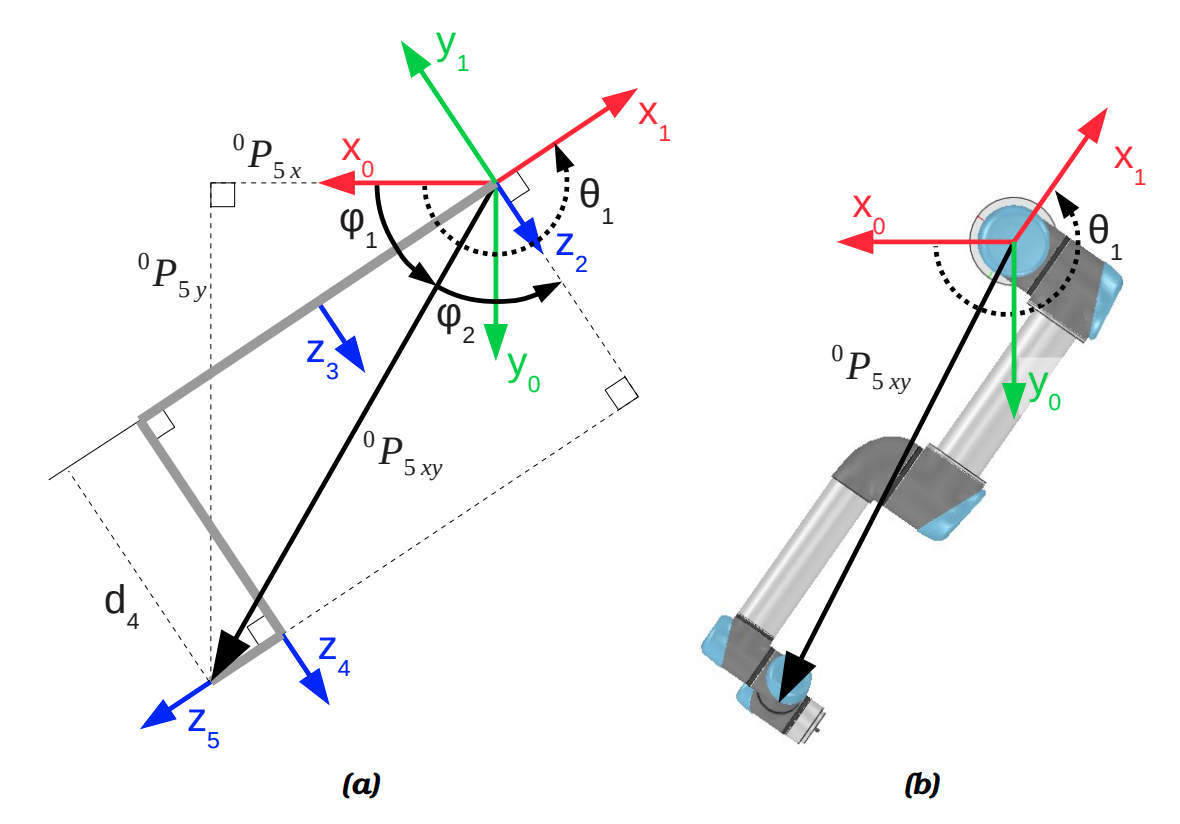
\includegraphics[width = .5\textwidth]{Bilder/inv1}
    \caption{Berechnung von $\theta_1$, Betrachtung von Gelenk eins bis fünf~\cite{rasmusandersenKinematicsUR52018}}\label{fig:inv1-1}
\end{figure}

\subsubsection{2. Gelenk fünf (oberes Handgelenk)}

Im Anschluss kann $\theta_5$ bestimmt werden, da der y-Teil der Position von Gelenk 6 relativ zu Gelenk 1 ($P_{1,6y}$) nur mithilfe von $\theta_5$ und bereits bekannter Parameter $P_{0,6}$, $\theta_1$ und der DH-Parameter berechnet werden kann (siehe Abbildung~\ref{fig:inv1-2}).
Aus dieser Erkenntnis ergibt sich Gleichung~\ref{eq:inv2-1}
$P_{1,6y}$ erhält man durch die Rotation des Ursprungssystems $T_{0,6}$ um die $z_1$-Achse (Gleichung~\ref{eq:inv2-2}).
In Kombination erhält man die Gleichung für $\theta_5$ (Gleichung~\ref{eq:inv2-3}).
Dabei entstehen wiederum zwei Lösungen, die jeweils das Handgelenk ober- oder unterhalb des Arms platzieren.
\begin{equation}
    - P_{1,6y} = d_4 + d_6 \cdot \cos(\theta_5)
    \label{eq:inv2-1}
\end{equation}
\begin{equation}
    P_{1,6y} = - P_{0,6x} \cdot \sin(\theta_1) + P_{0,6y} \cdot cos(\theta_1)
    \label{eq:inv2-2}
\end{equation}
\begin{equation}
    \theta_5 = \pm \arccos \left( \frac{ P_{0,6x} \cdot \sin\theta_1 - P_{0,6y} \cdot \cos\theta_1 - d_4 }{ d_6 } \right)
    \label{eq:inv2-3}
\end{equation}
\begin{figure}[h]
    \centering
    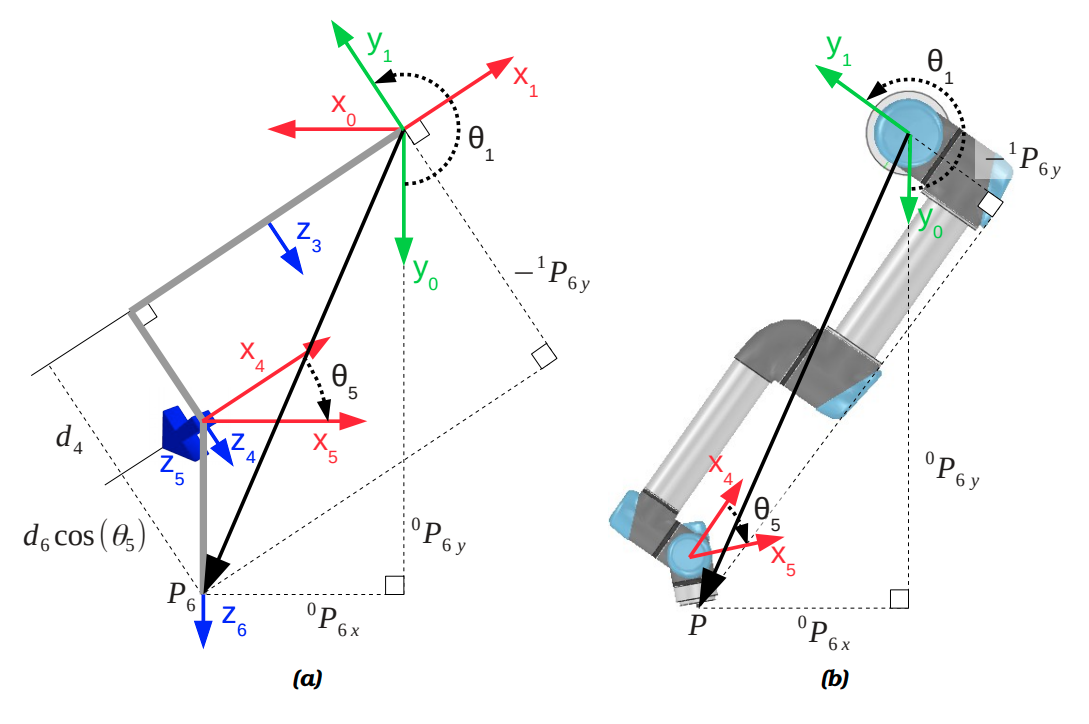
\includegraphics[width = .5\textwidth]{Bilder/inv2}
    \caption{Berechnung von $\theta_5$, Betrachtung von allen Gelenken~\cite{rasmusandersenKinematicsUR52018}}\label{fig:inv1-2}
\end{figure}

\subsubsection{3. Gelenk sechs (Endeffektor)}

Nach $\theta_1$ und $\theta_5$ wird $\theta_6$ bestimmt.
Dazu wird die Eigenschaft des UR5 herangezogen, die Z-Achsen von Gelenken zwei, drei und vier liegt stets parallel zur Y-Achse von Gelenk 1 stehen (siehe Abbildung~\ref{fig:ur5-axis}).
Deshalb kann die Y-Achse $y_1$ beschrieben von Gelenk sechs ($Y_{6,1}$) unabhängig von $\theta_{1,2,3,4}$ und kann mithilfe von sphärischen Koordinaten als $-Y_{6,1}(-\theta_6,\theta_5)$ ($-\theta_5$ als Azimuth sowie $\theta_6$ als polaren Winkel) aufgefasst werden (Abbildung~\ref{fig:inv1-3}).
Eine Umrechnung in kartesische Koordinaten ergibt deshalb Gleichung~\ref{eq:inv3-1}, wobei $Y_{6,1}$ mithilfe einer Drehung um $\theta_1$ um $z_1$ beschrieben werden kann (Gleichung~\ref{eq:inv3-2}).
$Z$ und $X$ sind hierbei jeweils Einheitsvektoren der Z- und X-Achse des jeweiligen Koordinatensystems.
Nach Gleichsetzen der x- und y-Einträge der beiden Gleichungen und anschließendem Umformen erhält man $\theta_6$ (Gleichung~\ref{eq:inv3-3}).
Dabei kann es genau eine Lösung geben.
Falls $\sin\theta_5=0$, liegt eine Singularität vor und eine Lösung kann nicht bestimmt werden.
Dies tritt auf, wenn neben den Achsen $z_2$, $z_3$ und $z_4$ auch Achse $z_6$ parallel steht.
\begin{figure}[h]
    \centering
    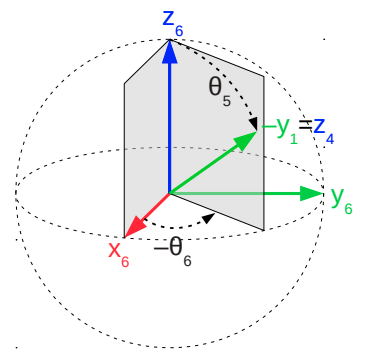
\includegraphics[width = .4\textwidth]{Bilder/inv3}
    \caption{Berechnung von $\theta_6$ mit Sphärischen Koordinaten, für Koordinatensystembeschreibung siehe Abbildung~\ref{fig:ur5-axis}}\label{fig:inv1-3}
\end{figure}
\begin{equation}
    Y_{6,1}=
    \begin{bmatrix}
        -\sin\theta_5 \cdot \cos\theta_6 \\ \sin\theta_5 \cdot\sin\theta_6 \\ -\cos\theta_5
    \end{bmatrix}
    \label{eq:inv3-1}
\end{equation}
\begin{equation}
    Y_{6,1}=
    -\sin\theta_1\cdot X_{6,0} + \cos\theta_1\cdot Y_{6,0}
    \label{eq:inv3-2}
\end{equation}
\begin{equation}
    \theta_6=
    \arctantwo\left(
    \frac{
        -X_{6,0y} \cdot \sin\theta_1 + Y_{6,0y} \cdot \cos\theta_1
    }{
        \sin\theta_5
    },
    \frac{
        X_{6,0x} \cdot \sin\theta_1 - Y_{6,0x} \cdot \cos\theta_1
    }{
        \sin\theta_5
    }\right)
    \label{eq:inv3-3}
\end{equation}

\subsubsection{4. Gelenk drei (Ellenbogen)}

Die verbleibenden drei Gelenke haben alle parallele Achsen und lassen sich dadurch zu einem zweidimensionalen System vereinfachen (siehe Abbildung~\ref{fig:inv1-4}, rechts).
Um $\theta_3$ zu berechnen kann der Winkel $\phi_3$ zu Hilfe genommen werden (siehe Gleichung~\ref{eq:inv4-1}).
Die Werte $a_2$, $a_3$ sind dabei die DH-Parameter der jeweiligen Gelenke und $\lvert P_{1,4xz} \rvert$ ist der Abstand zwischen Gelenk 1 und Gelenk 4, dessen relative Position bereits bekannt ist.
Aufgrund der Geometrie gilt: $\lvert P_{1,4xz} \rvert \in \lvert a_2 \pm a_3 \rvert$
Nach der Anwendung des $\arccos$ erhält man in der Regel zwei Lösungen, die der Position \enquote{Elbow Up} und \enquote{Elbow Down} entsprechen (Gleichung~\ref{eq:inv4-2}).
\begin{equation}
    \cos(\theta_3) = -cos(\phi_3) = \frac{a_2^2 + a_3^2 - \lvert P_{1,4xz}^2 \rvert}{2 a_2 a_3}   \label{eq:inv4-1}
\end{equation}
\begin{equation}
    \theta_3 = \pm \arccos \left(  \frac{a_2^2 + a_3^2 - \lvert P_{1,4xz}^2 \rvert}{2 a_2 a_3} \right)  \label{eq:inv4-2}
\end{equation}
\begin{figure}[h]
    \centering
    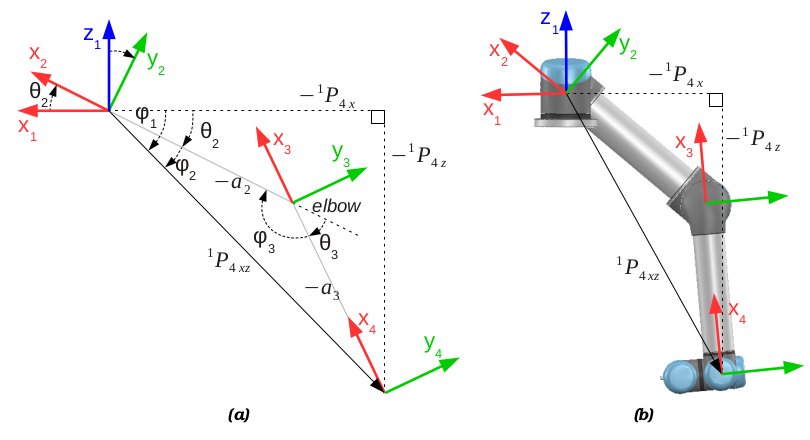
\includegraphics[width = .8\textwidth]{Bilder/inv4}
    \caption{Berechnung von $\theta_4$ durch Vereinfachung als zweidimensionales System und Bestimmung der Transformation zwischen Gelenk 1 und Gelenk 4.}\label{fig:inv1-4}
\end{figure}

\subsubsection{5. Gelenk zwei (Schulter)}

$\theta_2$ kann mithilfe von Abbildung~\ref{fig:inv1-4} ($\theta_2 = \phi_1 - \phi_2$), sowie Gleichung~\ref{eq:inv5-2} und ~\ref{eq:inv5-3} bestimmt werden.
Nach der Substitution von $\phi_3 = \sin(\pi-\theta_3) = \sin(\theta_3)$ erhält man eine Lösung für $\theta_2$ (Gleichung~\ref{eq:inv5-4}).
%\begin{equation}
%    \label{eq:inv5-1}
%\end{equation}
\begin{equation}
    \phi_1 = \arctantwo(-P_{1,4_z}, -P_{1,4x}) \label{eq:inv5-2}
\end{equation}
\begin{equation}
    \phi_2 = \arcsin\left( \frac{-a_3\cdot \sin \phi_3}{\lvert P_{1,4xz}\rvert} \right) \label{eq:inv5-3}
\end{equation}
\begin{equation}
    \theta_2 = \phi_1 - \phi_2 =
    \arctantwo(-P_{1,4_z}, -P_{1,4x}) -
    \arcsin\left( \frac{-a_3\cdot \sin \theta_3}{\lvert P_{1,4xz}\rvert} \right)
    \label{eq:inv5-4}
\end{equation}

\subsubsection{6. Gelenk vier (unteres Handgelenk)}

Der Winkel des letzten Gelenks ist definiert als der Winkel zwischen den Achsen $x_3$ und $x_4$ um Rotationsachse $z_4$ (siehe Definition DH-Parameter, Abschnitt~\ref{sec:dh-konvention}).
Da alle anderen Winkel bereits bekannt sind, kann der letzte Winkel der ersten Spalte $X_{3,4}$ der Transformationsmatrix $T_{3,4}$ entnommen werden.
Mit den ersten beiden Werten dieser Spalte, $X_{3,4x}$ und $X_{3,4y}$, erhält man den Wert von $\theta_4$ (Gleichung~\ref{eq:inv6-1})

\begin{equation}
    \theta_4 = \arctantwo\left( X_{3,4y}, X_{3,4x} \right)    \label{eq:inv6-1}
\end{equation}

\subsubsection{Zusammenfassung}

Mithilfe der Gleichungen~\ref{eq:inv7-1} bis~\ref{eq:inv7-6} kann die Inverse Kinematik eines UR5-Roboters direkt bestimmt werden.
Dabei existieren acht Lösungen, jeweils eine für die Gelenke sechs (Endeffektor), zwei (Schulter) und vier (unteres Handgelenk) und jeweils zwei für die Gelenke eins (Basis), drei (Ellenbogen) und fünf (oberes Handgelenk).
Neben den DH-Parametern und der gewünschten Transformation des Endeffektors muss für Gleichung~\ref{eq:inv7-1} $P_{0,5}$ (siehe Gleichung~\ref{fig:inv1-1}), für Gleichung~\ref{eq:inv7-3} die Einheitsvektoren $X_{6,0x}$, $X_{6,0y}$ und $Y_{6,0x}$ $Y_{6,0x}$, für Gleichung~\ref{eq:inv7-4} und~\ref{eq:inv7-4} die x- und y-Werte des Vektors $P_{1,4}$ und für Gleichung~\ref{eq:inv7-6} die Werte $(1,1)$ und $(2,1)$ der Transformationsmatrix $T_{3,4}$ bestimmt werden.

\begin{equation}
    \theta_1 = \arctantwo(P_{0,5y}, P_{0,5x}) \pm \arccos \left( \frac{d_4}{ \sqrt{ P_{0,5x}^2 + P_{0,5y}^2 }  } \right) + \frac{\pi}{2}
    \label{eq:inv7-1}
\end{equation}
\begin{equation}
    \theta_5 = \pm \arccos \left( \frac{ P_{0,6x} \cdot \sin\theta_1 - P_{0,6y} \cdot \cos\theta_1 - d_4 }{ d_6 } \right)
    \label{eq:inv7-2}
\end{equation}
\begin{equation}
    \theta_6 =
    \arctantwo\left(
    \frac{
        -X_{6,0y} \cdot \sin\theta_1 + Y_{6,0y} \cdot \cos\theta_1
    }{
        \sin\theta_5
    },
    \frac{
        X_{6,0x} \cdot \sin\theta_1 - Y_{6,0x} \cdot \cos\theta_1
    }{
        \sin\theta_5
    }\right)
    \label{eq:inv7-3}
\end{equation}
\begin{equation}
    \theta_3 = \pm \arccos \left(  \frac{a_2^2 + a_3^2 - \lvert P_{1,4xz}^2 \rvert}{2 a_2 a_3} \right)
    \label{eq:inv7-4}
\end{equation}
\begin{equation}
    \theta_2 = \phi_1 - \phi_2 =
    \arctantwo(-P_{1,4_z}, -P_{1,4x}) -
    \arcsin\left( \frac{-a_3\cdot \sin \theta_3}{\lvert P_{1,4xz}\rvert} \right)
    \label{eq:inv7-5}
\end{equation}
\begin{equation}
    \theta_4 = \arctantwo\left( X_{3,4y}, X_{3,4x} \right)
    \label{eq:inv7-6}
\end{equation}


\section{Singularitäten}\label{sec:singularitaten}


Kuka vs UR5.

Theorie (rundungsfehler), Praxis (große Geschwindigkeiten)
alpha-2
alpha-1
alpha-5
Elbow-Up / Elbow-Down


\section{Geschwindigkeitskinematik}